\documentclass[tikz,margin=2mm]{standalone}
\usepackage{amsmath}


\usetikzlibrary{trees,arrows}


\begin{document}

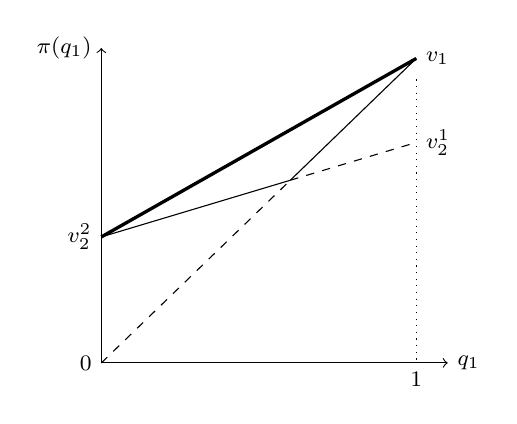
\begin{tikzpicture}[domain=0.001:1, scale=4, xscale=1, font=\footnotesize] 
        %% v = 1, c_s = 0.4, c_m = 0.2
  		%% vertices
    	\draw[->] (0, 0) node[left]{$0$} -- (1.1, 0) node[right] {$q_1$}; 
    	\draw[->] (0, 0) -- (0, 1) node[left] {$\pi(q
    	_1)$};
    	%% 
    	\draw[very thick] (0, 0.4) -- (1, 0.58/0.6);
    	\draw[] (0.6, 0.58) -- (1, 0.58/0.6) node[right]{$v_1$};
    	\draw[dashed] (0, 0) -- (0.6, 0.58);
    	\draw[] (0, 0.4) node[left]{$v_2^2$} -- (0.6, 0.58);
    	\draw[dashed] (0.6, 0.58) -- (1, 0.7) node[right]{$v_2^1$}; 
    	\draw[dotted] (1, 0.9) -- (1, 0) node [below]{$1$}; 
\end{tikzpicture}
       	
\end{document}